\chapter{Problème d'inversion adapté à la mesure}
\minitoc

\section{Definition d'un problème d'inversion}


\section{Mesure d'impulsions attosecondes par une approche "Frog"}


\section{Generalité sur l'inversion à 1 dimension}

\begin{figure}[!h]
\centering
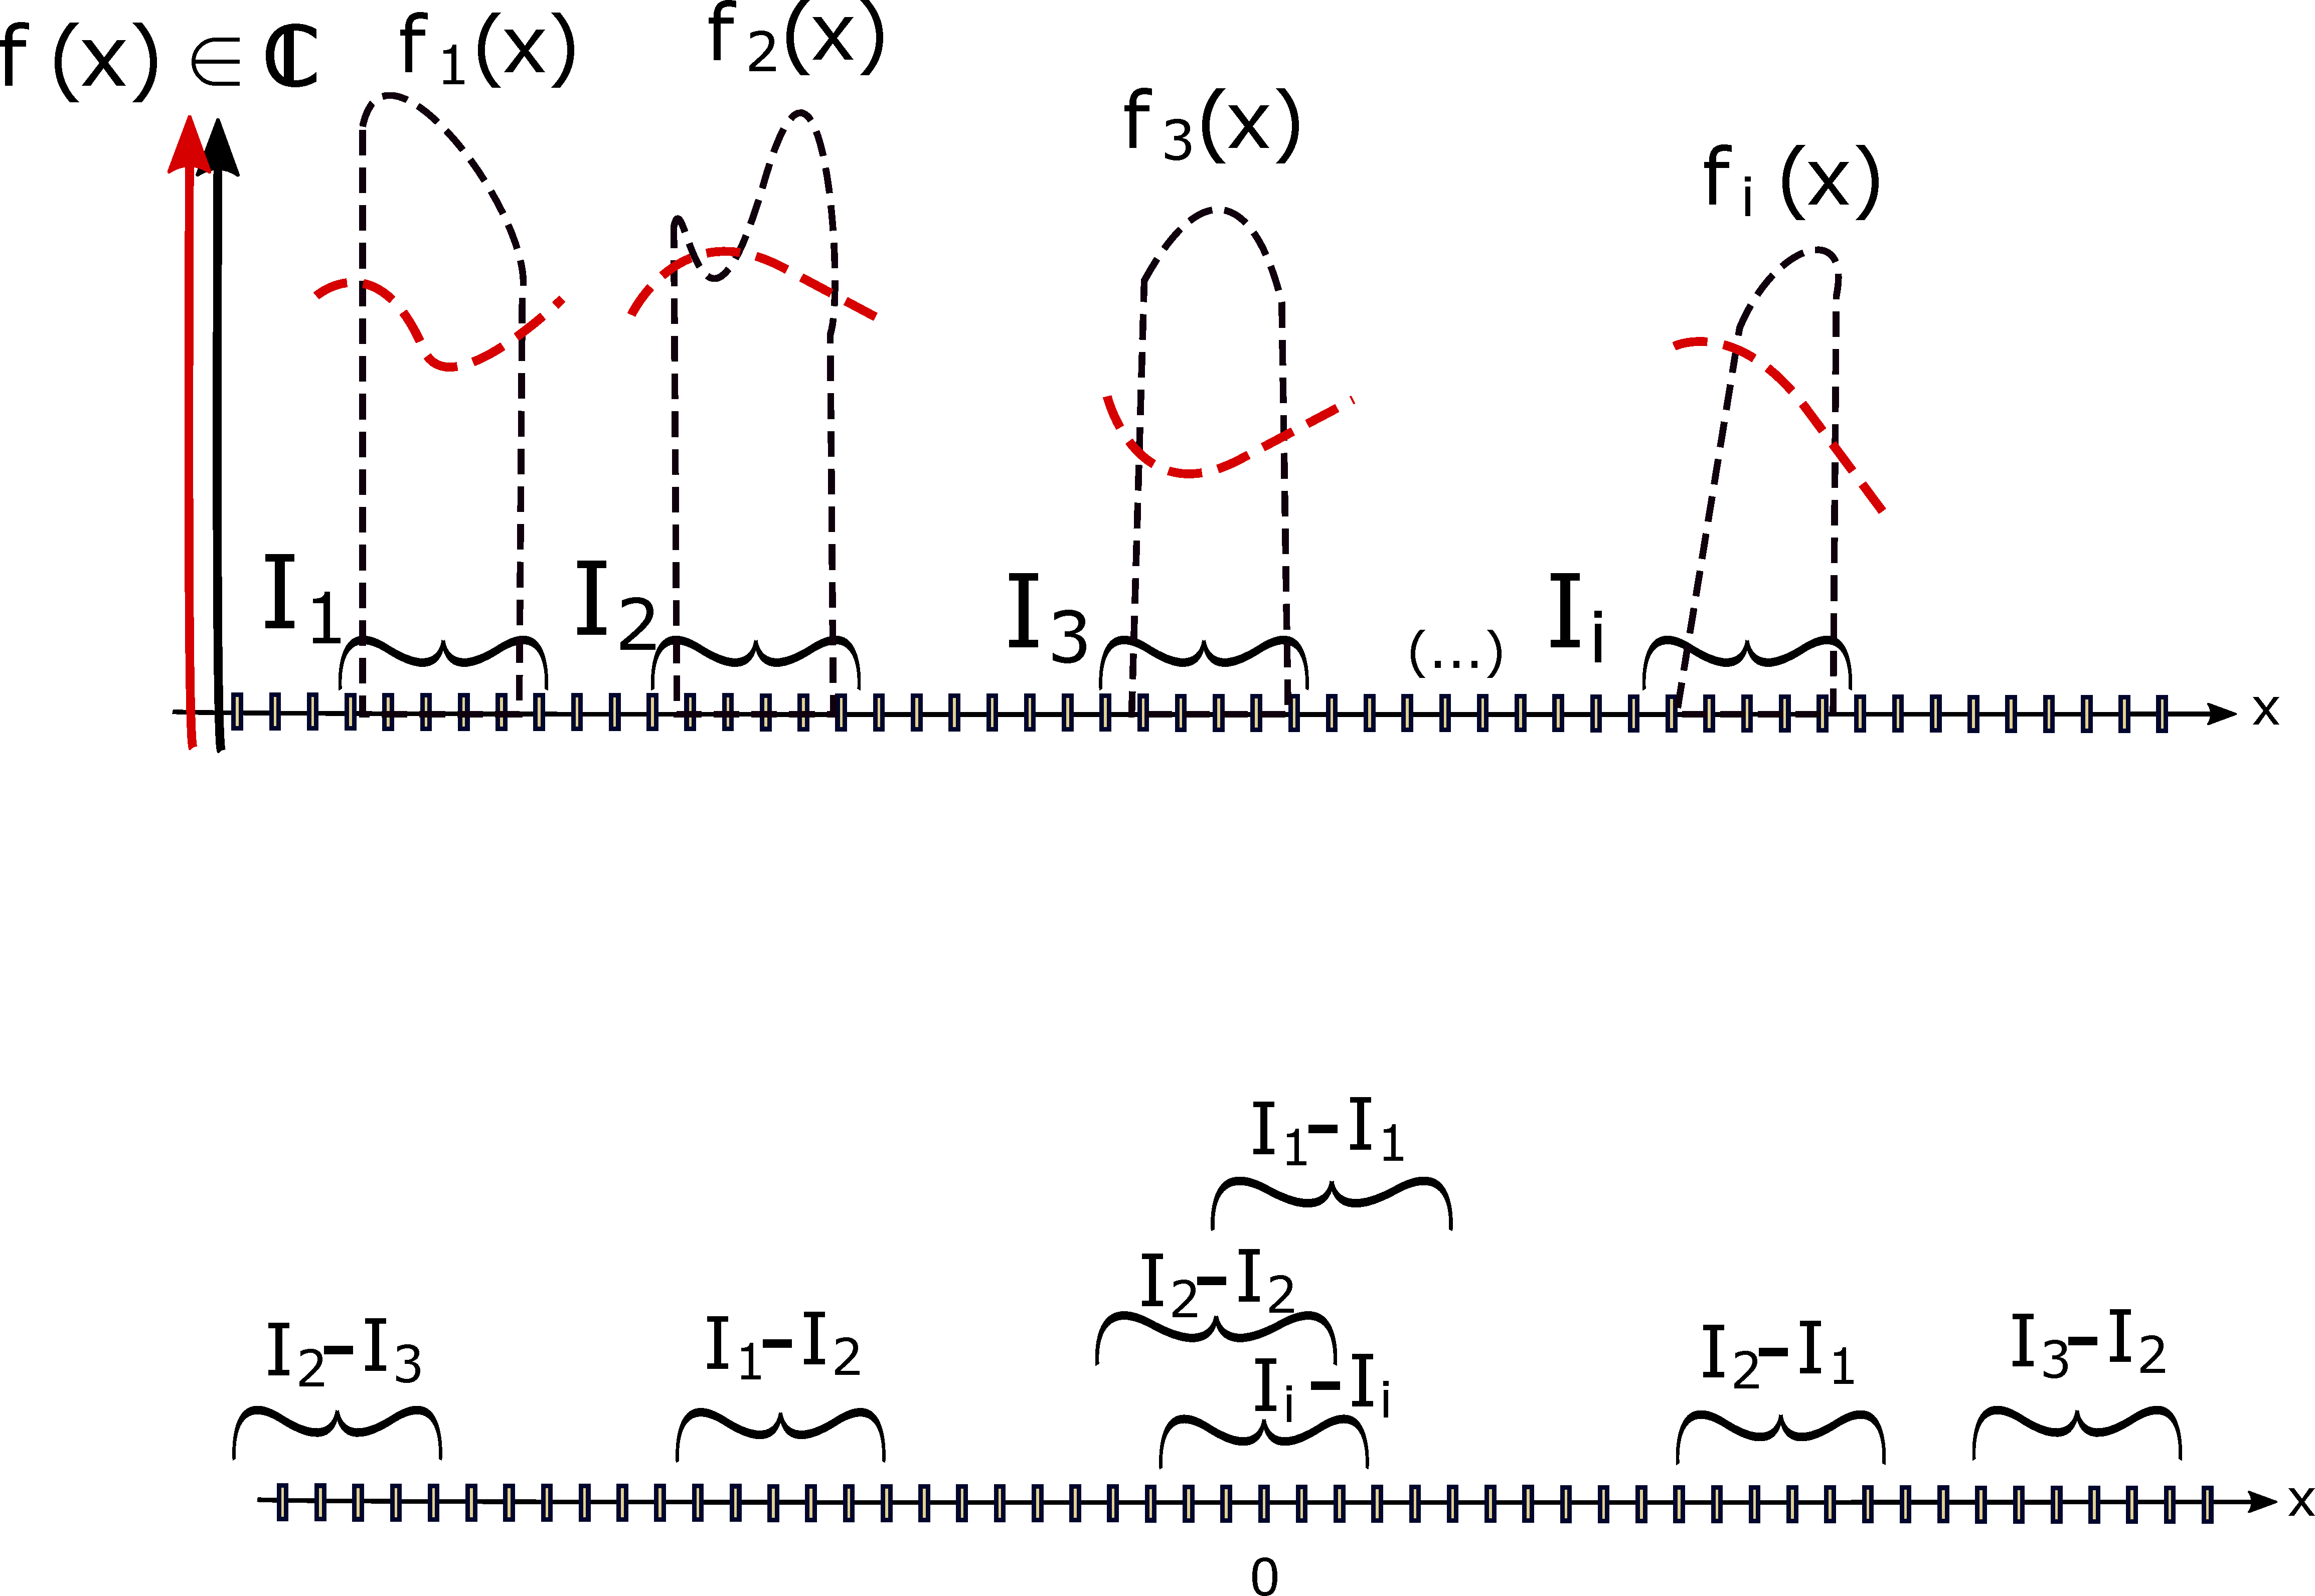
\includegraphics[width =0.8\textwidth]{../chapitre5/images/intervalleDisjoint.pdf}\\
\caption{\label{fig:intervalleDisjoint}}
\end{figure}

We define:
\begin{equation}
I_m - I_n=\{  x-y: x\in I_m,y\in I_y \}
\end{equation}

If the intervals $I_m - I_n$ are distinct as represented in Fig~\ref{fig:intervalleDisjoint}, than the inversion problem has one only solution \cite{crimmins1983uniqueness}.


The problem of phase retrival is to reconstruct $f(x)$ from the modulous $|F(\nu)|$ of its fourier transform :

\begin{equation}
F(\nu) = \int_{\mathbb{R}}f(x)e^{-i\nu x}dx
\end{equation}

For this problem, we define as equivalent to solutions $F(\nu)$ and $G(\nu)$ verifying
\begin{equation}
F(\nu) = e^{i(\alpha \nu+\beta)}G(\nu)
\end{equation}

where $\alpha,\beta \in \mathbb{R}$. The problem is therefore said to have a unique solution if all possible solutions are equivalent. An equivalent definition would be to say we have reconstructed $f(x)$ that a translation of $f(x)$ is still a solution as well as a multiplication by a constant phase. 

The importance of the fonction support can well be understood when one realizes the relation:

\begin{equation}
|F(\nu)|^2 = F(\nu)\overline{F(\nu)} = \int_{\mathbb{R}}[\int_{\mathbb{R}} f(u)\overline{f(x-u)}du]e^{-i\nu x}dx
\end{equation}

therefore, if $|F(\nu)| = |G(\nu)|$ we have necessarely (inversibility of the fourier transform) :

\begin{equation}
\int_{\mathbb{R}} f(u)\overline{f(x-u)}du= \int_{\mathbb{R}} g(u)\overline{g(x-u)}du
\end{equation}


The majority of work performed on this question of solution uniqueness are based on holomorphic functions theories. Without getting into the details of this mathmatical branch, lets recall some very usefull theorme traduced in ``understable terms'' which will rely on:

The Schwartz's Paley–Wiener theorem asserts that the fourier transform of a function with a compact support defined on $\mathbb{R}^n$ is entire on $\mathbb{C}^n$. In other word, since all of our fourier transform are applied on field located on a finit region of space (= compact support), we can say without risk that the funtion $F(\nu)$ defined above is entire. 

If $|f(z)|<e^{|z|^{\alpha}}$, $f$ is saif to be of order $\alpha$.

This will allow us to use Hadamard theorem:

Hadmard factorisation:
\begin{equation}
F(\nu) = e^{i(\alpha_0+\alpha_1 u)}\nu^m\prod_{k}^{\infty}(1 - \frac{\nu}{\nu_k})e^{\nu/\nu_k}
\end{equation}






\section{Algoritme de reconstruction pour la mesure de l'expansion du gradient}

